\RequirePackage[l2tabu, orthodox]{nag}
\documentclass[12pt]{article}

\usepackage[margin=1.9cm, letterpaper]{geometry}
\usepackage[utf8]{inputenc}
\usepackage{siunitx}
\usepackage{multicol}
\usepackage{mathtools}
\usepackage{amssymb}
\usepackage{mathrsfs}
\usepackage{graphicx}
\usepackage{float}
\usepackage[outputdir=obj]{minted}
\usepackage{pdflscape}
\usepackage{caption}
\usepackage{subcaption}
\usepackage{epstopdf}
\usepackage{pgfplots}
\usepackage{pgfplotstable}
\usepackage{pdfpages}
\usepackage{indentfirst}
\usepackage{parskip}

\epstopdfsetup{outdir=./obj/}
\usemintedstyle{emacs}
\setminted{linenos,breaklines}

\setlength{\parskip}{1em}
\setlength{\parindent}{2em}

\pgfplotsset{compat=1.17}

\title{Dual Rail Power Supply design\\ECE 302 Lab \#1}
\author{Hans Jarales (1537516) Michael Kwok (1548454)}
\date{October 14, 2020}
\begin{document}
\begin{titlepage}
\maketitle
\section*{Abstract}
The design of a regulated DC dual rail power supply with the specifications provided is an exercise in both knowledge of electrical circuits and the ability to apply it. The goal was to produce a regulated \(\pm\) \SI{10}{\volt} power supply with a stable output of \SI{25}{\milli\ampere} to resistive loads, 5\% voltage regulation and a maximum ripple of 0.5\% from an input of \(120\si{\volt}_{rms}\). This was done in four stages; the transformer stage, rectification stage, filter stage and finally the regulation stage.

The transformer used was a center tapped transformer. The rectification stage was a full-wave bridge rectifier utilizing 4 diodes to give us a full DC signal for each rail. A low-pass filter was used to smooth out the circuit, turning it from a cyclic signal to one that appears flat. For voltage regulation, a Zener diode in reverse bias mode was used, resulting in a stable voltage with a minimum current.
% TODO: Insert ripple and voltage regulation numbers

Our signatures certify that we are submitting our own, original work only, and do so in accordance with the University Code of Student Behaviour and APEGA's Code of Ethics.


\includegraphics[width=0.2\linewidth]{hanssignature.png}

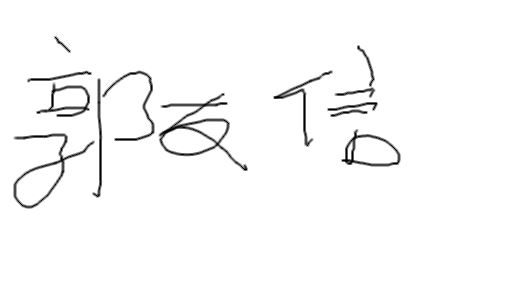
\includegraphics[width=0.2\linewidth]{bepis.png}
\end{titlepage}
\newpage
\section{Objectives}
The purpose of this project was to create a Dual Rail $\pm10V$, and $\pm 9V$ regulated DC Power Supply -- with the following goals:
\begin{itemize}
    \item Supplies 25mA to both loads independently,
    \item Allow a maximum of 0.5\% ripple on the output voltage,
    \item Provide voltage regulation of less than 5\% (no-load voltage).
\end{itemize}

A simplified block diagram is shown in Figure \ref{fig:blockDiagram}.

\begin{figure}
    \centering
    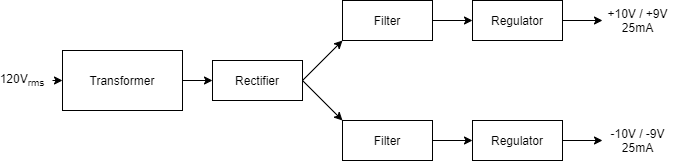
\includegraphics[width = \textwidth]{302Lab1BlockDiagram.png}
    \caption{Simplified Block Diagram of Dual Rail Power Supply}
    \label{fig:blockDiagram}
\end{figure}

\section{Design}
The project was designed in 4 stages or modules, with the following stages in order:
\begin{enumerate}
    \item Transformer
    \item Rectifier
    \item Filter
    \item Regulator
\end{enumerate}
This modularity with the design gave us the ability to improve and debug each part separately. The transformer was provided as a single unit, and so not much about it will be described other than calculation. 

The transformer allows us to step down the voltage from $120\si{\volt}_rms$ to $42.5\si{\volt}_{pk}$ which is easier to manage.

In the rectification stage, the previously stepped down voltage passed a Full-Wave bridge rectifier design to appropriately convert AC to DC with the correct bias for each rail.

By applying a Low-Pass Filter to the previous output, the wave-like voltage output was ``straightened'' to produce an almost constant voltage of roughly \SI{22}{\volt} instead of a wave-like voltage.

Using a Zener diode based voltage regulation circuit, the 20V filtered output was cut down to the proper outputs required. Two different designs were made, one for $\pm 9\si{\volt}$ and another for $\pm 10\si{\volt}$, thus requiring two different ballast resistances and target currents.

\subsection{Transformer Stage}
The power supply utilizes the standard wall outlet; therefore a voltage of $120V_{rms}$ ($170V_{pk}$) at 60Hz is experienced at the input of the power supply. In order to separate the voltage into a positive and negative rail, a center-tapped step-down transformer (\textbf{Hammond Type C, Model 166D25}) with a 4:1 voltage reduction ratio is implemented. With such a ratio, the center-tapped transformer further divides the secondary voltage in half. The resulting voltage(s) on the secondary side is then: 
\[ \frac{170V_{pk}}{4} = 42.5V_{pk}\]
Where each rail is a \SI{60}{\hertz} sinusoidal wave with a peak to peak voltage of \SI{42.5}{\volt} with respect to ground.
The transformer is assumed to have some internal resistance; \SI{0.1}{\ohm} and \SI{18}{\ohm} is assumed at the primary and secondary side, respectively.

\subsection{Rectifier Stage}
A rectifier is a circuit that converts an AC signal input into a purely DC signal. At this stage, an efficient, non-costly rectifier solution is required.

In a Half-Wave rectifier, the resulting output signal is a pulsating DC signal; the positive half-cycles of a sinusoidal AC signal. However, this is inefficient for our design, as such a design only rectifies every positive half-cycle.

Like the Half-Wave rectifier, the Full-Wave rectifier outputs a pulsating DC signal, however, both positive and negative half-cycles of the oscillating AC signal are taken into account, making such a design more efficient than the previous consideration. However, such a rectifier design requires a more costly, center-tapped transformer.

The Full-Wave Bridge rectifier outputs a signal akin to the Full-Wave rectifier, while allowing both rails to be rectified without extra effort, and was therefore the best option for our design. The diode bridge consists of 4 diodes, acting in a way such that for each rail, only two diodes are active at a given time, whilst the remaining diodes are under \textit{reverse bias}, blocking current entering the anode. As the signal from the Transformer stage oscillates, the paths for which the current enters the diode bridge alternate, however, the orientation/direction in which the current enters the remaining Filter, and Regulator stage(s) remain the same, resulting in the same voltage polarities throughout the duration of operation.

\subsubsection{Testing}
This stage was tested with a \SI{1}{\kilo\ohm} load attached between the output and ground. The simulation and testing was done in SPICE software, namely LTSpice and ngspice.
%TODO fill out more

\subsection{Filter Stage}
A capacitor parallel to the output signal was used to buffer the incoming unstable DC signal. As the DC signal rises, the capacitor begins to store energy. As soon as the signal begins to decrease (the instant after the peak), the capacitor begins to gradually release the stored energy. This gradual release counteracts the declining DC signal, until it rises again. This layout of the circuit produced a low pass filter, which produced an output signal that appeared ``flattened'' -- the original signal removed of the sharp inclines and declines after the initial charge time. A high pass filter would not reduce the frequency of the output signal. Band pass filters would not be useful in our case as we would like the output frequency to be as close to 0 as possible.

A \SI{100}{\micro\farad} Capacitor was chosen for both rails. A higher capacitance, or additional parallel capacitors, produces an output signal with approximately the same ripple voltage, however, the output signal will have a slower charge time, as the capacitance is higher, requiring more time to reach a stable output. A smaller capacitance results in an output signal with higher ripple voltage. The capacitance chosen had a good trade-off between charge time and voltage. Where the voltage across the capacitor contains a superimposed ripple, the capacitor voltage $V_C$ was taken as the voltage at the lower magnitude peak.

\subsubsection{Testing}

This stage was tested to calculate the ripple voltage and the voltage when loaded compared to unloaded. A \SI{1000}{\ohm} resistor was used to simulate a load and get a baseline number for our analysis.

The measured ripple for the positive rail is expected to be:
$$V_r = \frac{I_b}{2\pi f C} = \frac{27.5mA}{2\pi (60Hz)(100\mu F} = 0.729V$$
\begin{align*}
    V_{pk} &= \left|V_{max} - V_{min}\right|\\
    \left|19.13757 - 20.28665\right| &= 1.14908
\end{align*}
And with the same formula for the negative rail, it was also \(1.14908\). Both values are below the requirement of \SI{1.5}{\volt} in the filtering stage.

The average voltage for the loaded circuit after filtering was calculated to be \(19.72689189\).

Previous results were calculated with 1657 data points of the simulated values from \SI{0.02}{\second} up to \SI{1}{\second}. The initial delay is to allow for the system to stabilize and charge up.

\subsection{Regulator Stage}
The regulator stage takes the cleaned up signal from the filtering stage and ensures that it can output a set voltage for any load. At the same time, ripple can be improved due to the use of the Zener diode in our regulator design.

A Zener diode in \textit{reverse bias} is in a state of ~0A (close to an open circuit) until a certain voltage is achieved. Beyond this voltage, the diode enters breakdown. This voltage, denoted as $V_z$ (\textit{breakdown voltage}) when reached, remains constant across the diode, with little to no change as the current passing through the diode increases. The current corresponding to this voltage is denoted $I_{zk}$; any current greater than this produces the same voltage across the diode. Indeed, this makes the Zener diode a useful regulating device. It is placed across the load to produce the desired voltage output.\par
Diodes have a maximum power rating that allows us to use it before thermal overload. Power also is wasted and lost when too much current enters the Zener diode. The previous two reasons are why current entering the Zener diode is limited via a resistor, denoted as $R_{Ballast}$. The current through the diode at our lowest voltage is targeted at $I_z = 2.5mA$ to allow for good regulation characteristics. Determining the right value of $R_{Ballast}$ depends on the desired output voltage.
\begin{itemize}
    \item For the +10V output:
    $$R_{Ballast} = \frac{V_C - 10V}{I_R} = \frac{18.32V - 10V}{I_{Load} + I_z} = \frac{8.32V}{25mA + 2.5mA} \approx 303\Omega$$
    
    \item For the +9V output:
    $$R_{Ballast} = \frac{18 - 9V}{27.5mA} \approx 327\Omega$$
\end{itemize}

The calculation for the negative rails are similar, and have the same values.

\begin{figure}
    \centering
    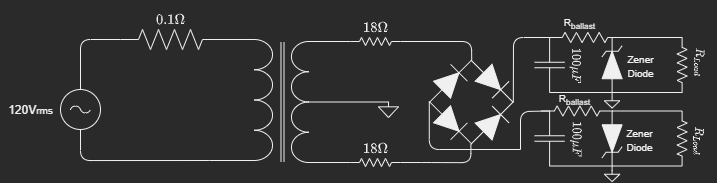
\includegraphics[width = \textwidth]{DualRailPSU.png}
    \caption{Full Circuit Schematic for Dual Rail Power Supply}
\end{figure}
\section{Simulation results}

All simulations are run from \(0 - 1\) seconds, and have a resolution of 0.1 ms. Some graphs truncated when the results stabilize and look the same, to allow for a more detailed view.

\subsection{9V simulation results}
\begin{tikzpicture}
    \begin{axis}[
        title = {Transformer input},
        xlabel = Time (\si{\second}),
        ylabel = Voltage (\si{\volt}),
        xmin = 0,
        xmax = 0.2,
        xmajorgrids,
        ymajorgrids,
        yminorgrids,
        width = {0.9\linewidth},
        height = {3.2in}]
    \addplot table [x=time, y=V(1), col sep=tab, mark=none] {tran.tsv};
    \end{axis}
\end{tikzpicture}

\begin{tikzpicture}
    \begin{axis}[
        title = {Transformer output},
        xlabel = Time (\si{\second}),
        ylabel = Voltage (\si{\volt}),
        xmin = 0,
        xmax = 0.2,
        xmajorgrids,
        ymajorgrids,
        yminorgrids,
        width = {0.9\linewidth},
        height = {3.2in}]
    \addplot table [x=time, y=V(5), col sep=tab, mark=none] {tran.tsv};
    \addplot table [x=time, y=V(6), col sep=tab, mark=none] {tran.tsv};
    \end{axis}
\end{tikzpicture}

\begin{tikzpicture}
    \begin{axis}[
        title = {Bridge rectified output},
        xlabel = Time (\si{\second}),
        ylabel = Voltage (\si{\volt}),
        xmin = 0,
        xmax = 0.2,
        xmajorgrids,
        ymajorgrids,
        yminorgrids,
        width = {0.9\linewidth},
        height = {4in}]
    \addplot table [x=time, y=V(7), col sep=tab, mark=none] {RectLoad.tsv};
    \addplot table [x=time, y=V(8), col sep=tab, mark=none] {RectLoad.tsv};
    \end{axis}
\end{tikzpicture}

\begin{tikzpicture}
    \begin{axis}[
        title = {Filter stage output with \SI{1000}{\ohm} load},
        xlabel = Time (\si{\second}),
        ylabel = Voltage (\si{\volt}),
        xmin = 0,
        xmax = 0.1,
        xmajorgrids,
        ymajorgrids,
        yminorgrids,
        width = {0.9\linewidth},
        height = {3.2in}]
    \addplot table [x=time, y=V(7), col sep=tab, mark=none] {FiltLoad.tsv};
    \addplot table [x=time, y=V(8), col sep=tab, mark=none] {FiltLoad.tsv};
    \end{axis}
\end{tikzpicture}

\begin{center}
\begin{tikzpicture}
    \begin{axis}[
        title = {+9v Regulated Output},
        xlabel = Time (\si{\second}),
        ylabel = Voltage (\si{\volt}),
        restrict x to domain = 0:0.03,
        xmin = 0,
        xmax = 0.025,
        ymin = 0,
        ymax = 10,
        xmajorgrids,
        yminorgrids,
        ymajorgrids,
        legend pos = south east,
        width = {0.9\linewidth},
        height = {2.0in}]
    \addplot table [x=time, y=V(9), col sep=tab, mark=none] {9vload.tsv};
    \addlegendentry{\SI{360}{\ohm} load}
    \addplot table [x=time, y=V(9), col sep=tab, mark=none] {9vunload.tsv};
    \addlegendentry{Unloaded}
\end{axis}
\end{tikzpicture}
\end{center}

\begin{center}
\begin{tikzpicture}
    \begin{axis}[
        title = {-9v Regulated Output},
        xlabel = Time (\si{\second}),
        ylabel = Voltage (\si{\volt}),
        restrict x to domain = 0:0.03,
        xmin = 0,
        xmax = 0.025,
        ymax = 0,
        ymin = -10,
        xmajorgrids,
        ymajorgrids,
        legend pos = north east,
        width = {0.9\linewidth},
        height = {2.0in}]
    \addplot table [x=time, y=V(10), col sep=tab, mark=none] {9vload.tsv};
    \addlegendentry{\SI{360}{\ohm} load}
    \addplot table [x=time, y=V(10), col sep=tab, mark=none] {9vunload.tsv};
    \addlegendentry{Unloaded}
\end{axis}
\end{tikzpicture}
\end{center}

Zoomed to show ripple:
\begin{center}
\begin{tikzpicture}
    \begin{axis}[
        title = {+9v Regulated Output with \SI{360}{\ohm} load},
        xlabel = Time (\si{\second}),
        ylabel = Voltage (\si{\volt}),
        restrict x to domain = 0.015:0.1,
        xmin = 0.02,
        xmax = 0.06,
        ymin = 9.02,
        ymax = 9.05,
        xmajorgrids,
        ymajorgrids,
        width = {0.9\linewidth},
        height = {1.8in}]
    \addplot table [x=time, y=V(9), col sep=tab, mark=none] {9vload.tsv};
\end{axis}
\end{tikzpicture}
\end{center}
\begin{center}
\begin{tikzpicture}
    \begin{axis}[
        title = {-9v Regulated Output with \SI{360}{\ohm} load},
        xlabel = Time (\si{\second}),
        ylabel = Voltage (\si{\volt}),
        restrict x to domain = 0.015:0.1,
        xmin = 0.02,
        xmax = 0.06,
        ymax = -9.02,
        ymin = -9.05,
        xmajorgrids,
        ymajorgrids,
        width = {0.9\linewidth},
        height = {1.8in}]
    \addplot table [x=time, y=V(10), col sep=tab, mark=none] {9vload.tsv};
\end{axis}
\end{tikzpicture}
\end{center}

\pagebreak
\subsection{10V simulation results}
\begin{tikzpicture}
    \begin{axis}[
        title = {Transformer input},
        xlabel = Time (\si{\second}),
        ylabel = Voltage (\si{\volt}),
        xmin = 0,
        xmax = 0.2,
        xmajorgrids,
        ymajorgrids,
        yminorgrids,
        width = {0.9\linewidth},
        height = {3.2in}]
    \addplot table [x=time, y=V(1), col sep=tab, mark=none] {tran.tsv};
    \end{axis}
\end{tikzpicture}

\begin{tikzpicture}
    \begin{axis}[
        title = {Transformer output},
        xlabel = Time (\si{\second}),
        ylabel = Voltage (\si{\volt}),
        xmin = 0,
        xmax = 0.2,
        xmajorgrids,
        ymajorgrids,
        yminorgrids,
        width = {0.9\linewidth},
        height = {3.2in}]
    \addplot table [x=time, y=V(5), col sep=tab, mark=none] {tran.tsv};
    \addplot table [x=time, y=V(6), col sep=tab, mark=none] {tran.tsv};
    \end{axis}
\end{tikzpicture}

\begin{tikzpicture}
    \begin{axis}[
        title = {Bridge rectified output},
        xlabel = Time (\si{\second}),
        ylabel = Voltage (\si{\volt}),
        xmin = 0,
        xmax = 0.2,
        xmajorgrids,
        ymajorgrids,
        yminorgrids,
        width = {0.9\linewidth},
        height = {4in}]
    \addplot table [x=time, y=V(7), col sep=tab, mark=none] {RectLoad.tsv};
    \addplot table [x=time, y=V(8), col sep=tab, mark=none] {RectLoad.tsv};
    \end{axis}
\end{tikzpicture}

\begin{tikzpicture}
    \begin{axis}[
        title = {Filter stage output with \SI{1000}{\ohm} load},
        xlabel = Time (\si{\second}),
        ylabel = Voltage (\si{\volt}),
        xmin = 0,
        xmax = 0.1,
        xmajorgrids,
        ymajorgrids,
        yminorgrids,
        width = {0.9\linewidth},
        height = {3.2in}]
    \addplot table [x=time, y=V(7), col sep=tab, mark=none] {FiltLoad.tsv};
    \addplot table [x=time, y=V(8), col sep=tab, mark=none] {FiltLoad.tsv};
    \end{axis}
\end{tikzpicture}

\begin{center}
\begin{tikzpicture}
    \begin{axis}[
        title = {+10v Regulated Output},
        xlabel = Time (\si{\second}),
        ylabel = Voltage (\si{\volt}),
        restrict x to domain = 0:0.03,
        xmin = 0,
        xmax = 0.025,
        ymin = 0,
        ymax = 11,
        xmajorgrids,
        yminorgrids,
        ymajorgrids,
        legend pos = south east,
        width = {0.9\linewidth},
        height = {2.0in}]
    \addplot table [x=time, y=V(9), col sep=tab, mark=none] {10vload.tsv};
    \addlegendentry{\SI{400}{\ohm} load}
    \addplot table [x=time, y=V(9), col sep=tab, mark=none] {10vunload.tsv};
    \addlegendentry{Unloaded}
\end{axis}
\end{tikzpicture}
\end{center}

\begin{center}
\begin{tikzpicture}
    \begin{axis}[
        title = {-10v Regulated Output },
        xlabel = Time (\si{\second}),
        ylabel = Voltage (\si{\volt}),
        restrict x to domain = 0:0.03,
        xmin = 0,
        xmax = 0.025,
        ymax = 0,
        ymin = -11,
        xmajorgrids,
        ymajorgrids,
        legend pos = north east,
        width = {0.9\linewidth},
        height = {2.0in}]
    \addplot table [x=time, y=V(10), col sep=tab, mark=none] {10vload.tsv};
    \addlegendentry{\SI{400}{\ohm} load}
    \addplot table [x=time, y=V(10), col sep=tab, mark=none] {10vunload.tsv};
    \addlegendentry{Unloaded}
\end{axis}
\end{tikzpicture}
\end{center}

Zoomed to show ripple:
\begin{center}
\begin{tikzpicture}
    \begin{axis}[
        title = {+10v Regulated Output with \SI{400}{\ohm} load},
        xlabel = Time (\si{\second}),
        ylabel = Voltage (\si{\volt}),
        restrict x to domain = 0.015:0.1,
        xmin = 0.02,
        xmax = 0.06,
        ymin = 9.97,
        ymax = 10,
        xmajorgrids,
        ymajorgrids,
        width = {0.9\linewidth},
        height = {1.8in}]
    \addplot table [x=time, y=V(9), col sep=tab, mark=none] {10vload.tsv};
\end{axis}
\end{tikzpicture}
\end{center}
\begin{center}
\begin{tikzpicture}
    \begin{axis}[
        title = {-10v Regulated Output with \SI{400}{\ohm} load},
        xlabel = Time (\si{\second}),
        ylabel = Voltage (\si{\volt}),
        restrict x to domain = 0.015:0.1,
        xmin = 0.02,
        xmax = 0.06,
        ymax = -9.97,
        ymin = -10,
        xmajorgrids,
        ymajorgrids,
        width = {0.9\linewidth},
        height = {1.8in}]
    \addplot table [x=time, y=V(10), col sep=tab, mark=none] {10vload.tsv};
\end{axis}
\end{tikzpicture}
\end{center}
\pagebreak
\section{Results}

The resulting ripple from the filter stage was measured to be the following:
\begin{align*}
    V_{pk} &= \left|V_{max} - V_{min}\right|\\
    \left|19.13757 - 20.28665\right| &= 1.14908
\end{align*}
And with the same formula for the negative rail, it was also \(1.14908\). Both values are below the requirement of \SI{1.5}{\volt} in the filtering stage.

Previous results were calculated with 1657 data points of the simulated values from \SI{0.02}{\second} up to \SI{1}{\second}. The initial delay is to allow for the system to stabilize and charge up.

The following calculation refers to the Voltage Regulation stage for the respective power supplies with values found via simulation:
\begin{itemize}
    \item 10V: \begin{align*}
        \frac{V_{No Load} - V_{Load}}{V_{No Load}} \cdot (100\%)&\\
        = \frac{10.009 - 9.9899}{10.009} \cdot (100\%)& = 0.191\%
    \end{align*}
\end{itemize}
\begin{itemize}
    \item 9v:\begin{align*}
    \frac{9.056978 - 9.040856}{V_{9.056978}} \cdot (100\%) = 0.178\%
    \end{align*}
\end{itemize}

The following Ripple Voltages $V_r$ were found:
\begin{itemize}
    \item 10V: $9.9899V - 9.9859V = 4mV$
    \item 9V: $9.040856 - 9.027528 = 13mV$
\end{itemize}

Indeed, simulations of the design achieved the criteria: the resulting ripple voltages met the required $V_r < 0.5\%$, or $V_r < 50mV$, and a voltage regulation better than 5\%; very close to ideal.

The measured ripple voltage at the capacitor filter from simulations:
\begin{align*}
    V_{pk} &= \left|V_{max} - V_{min}\right|\\
    \left|19.13757 - 20.28665\right| &= 1.14908
\end{align*}
And with the same formula for the negative rail, it was also \(1.14908\). Both values are below the requirement of \SI{1.5}{\volt} in the filtering stage.
Compared to the expected/theoretical value of 0.729V, a greater voltage when simulated suggests:
\begin{itemize}
    \item Higher $I_B$ than expected (\(\leq27.5mA\)),
    \item or a lower frequency than expected (\(\geq60Hz\)).
\end{itemize}

\section{Discussion}
\begin{enumerate}
    \item A low pass filter was used in this application. This is because we would like the resulting signal to be as close to \SI{0}{\hertz} as possible, and a high pass filter would counter that goal. Band filters could also be used, but require more components which will cause inefficiencies.
    \item No additional filtering was required in the final design as the ripple and regulation attained was within specification.
    \item A way to improve this design is to use a 78XX series IC for voltage regulation instead. Zener diode based regulation dissipates more power than an equivalent 7810/7809, which means that it is less efficient.
    \item There was a difference between the predicted voltage for filtering and the simulated voltage. This might be due to the simulations taking into account some parasitic losses in diodes or capacitors, and calculations being ``perfect world'' devices. Numerical discrepancies can also be due to the numerical methods that computers use to solve equations, such as the inductance for transformers.
    \item There were difficulties in finding the correct $R_{Ballast}$  in the regulator stage, in that relatively small differences in resistor values enlarged the output voltage ripple by a significant amount. To remedy this, ensure correct circuit connections so that the correct currents from the zener and the load should be made sure of, and most importantly the correct capacitor voltage $V_C$ measurements should be made.
\end{enumerate}

\section{Conclusions}
The design of efficient Dual Rail Power supply units take careful consideration in minimizing ripple voltage and enabling voltage regulation, while keeping in mind the desired output specifications. A strong knowledge and background in relevant areas (i.e. diodes, transformers, AC circuits) are essential in determining the best devices to use and in what order/combination -- which is essential in ultimately implementing the design. Additionally, concerning safety in the design of a power supply, prior simulations and theory should be rigorous before implementation. Simulations in the planning phase of the design process also help preemptively reveal certain issues or inefficiencies before implementation of the circuit. %A reduction in time with live current contact also reduces safety... %
 

\newpage

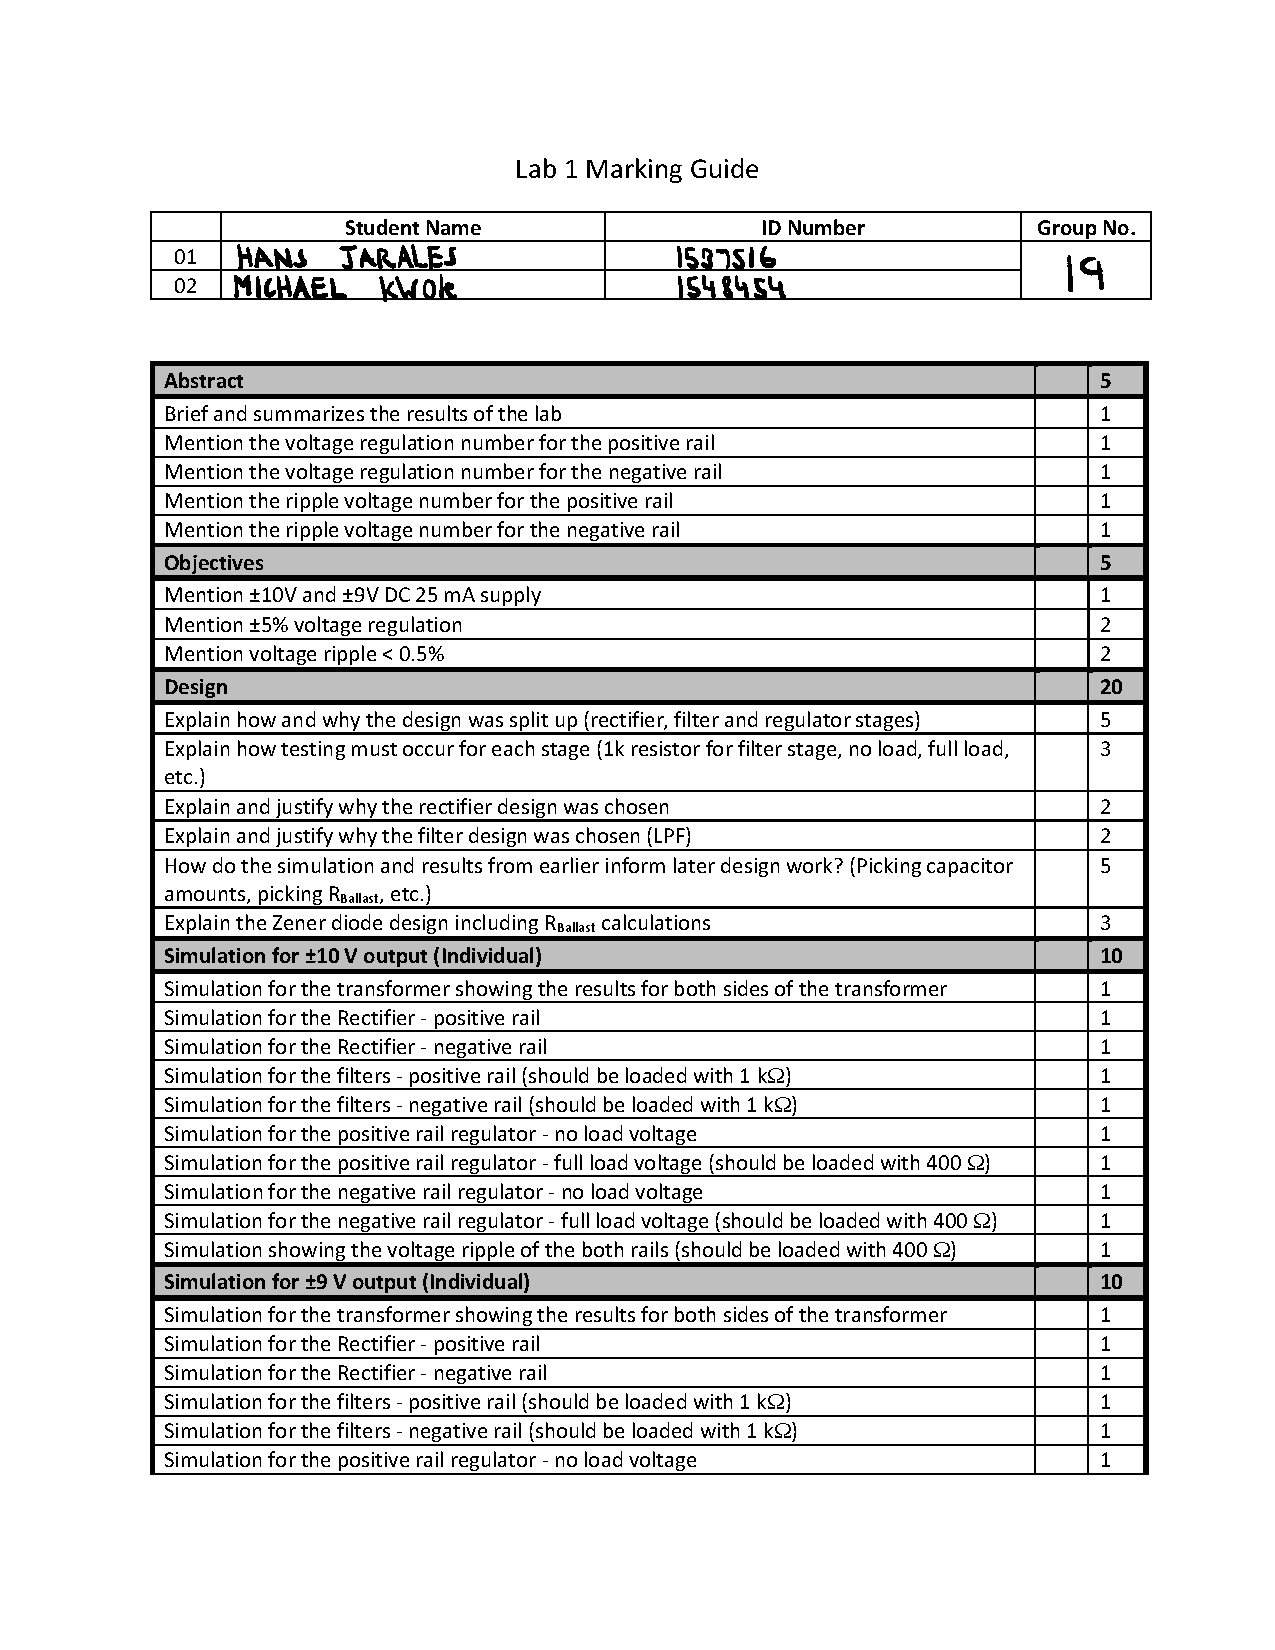
\includepdf[pages=-]{lab1markingsheet.pdf}
\end{document}
